\chapter{Introduction}

Nuclear physics aims to understand systems
where the structure and dynamics are dominated by the strong interaction,
one of the four fundamental forces of nature.
The goals of nuclear science are well-described by the overarching open questions
identified by the U.S.~National Academy of Science in \textit{Exploring the Heart of Matter}~\cite{NRC13heartofmatter}:
\begin{enumerate}
  \item How did matter come into being and how does it evolve?
  \item How does subatomic matter organize itself and what phenomena emerge?
  \item Are the fundamental interactions that are basic to the structure of matter fully understood?
  \item How can the knowledge and technological progress provided by nuclear physics best be used to benefit society?
\end{enumerate}
At the heart of this work is the second question,
with the focus of our attention being on the structure of atomic nuclei.

\begin{figure}[t]
  \centering
  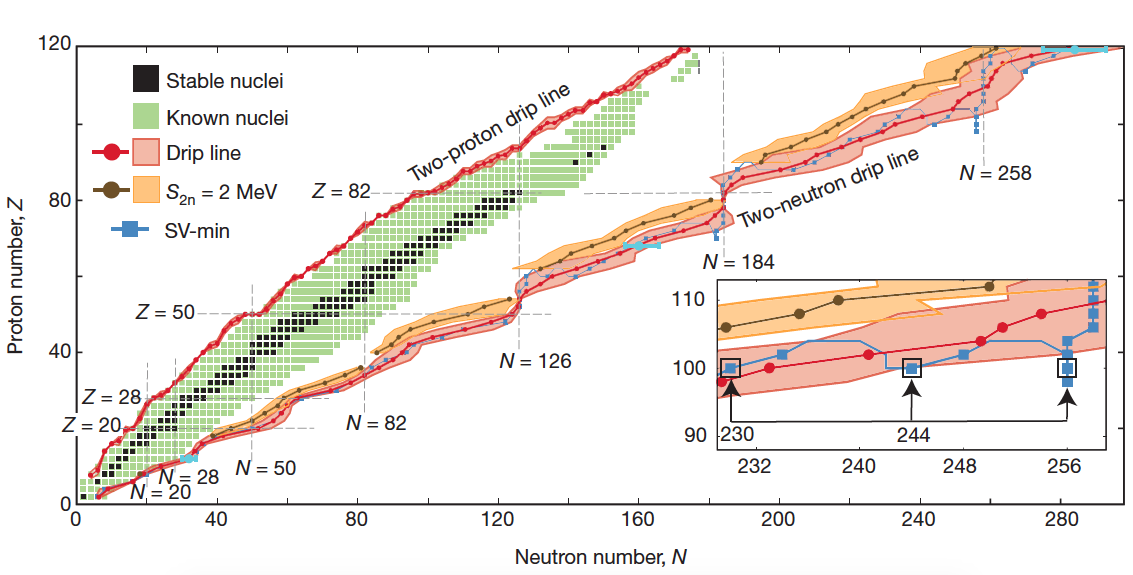
\includegraphics[width=1.0\textwidth]{proposal/doc/images/external/nuclear_landscape.png}
  \caption[
    The nuclear landscape,
    with stable and unstable atomic nuclei denoted by the black and green squares, respectively,
    and a theoretical prediction of the limit of bound nuclei being indicated by the red bands.
  ]{
    The nuclear landscape,
    with stable and unstable atomic nuclei denoted by the black and green squares, respectively,
    and a theoretical prediction of the limit of bound nuclei being indicated by the red bands.
    Figure taken from Ref.~\cite{Erle12limits}.
  }\label{fig:nuclear_landscape}
\end{figure}

Atomic nuclei consist of protons and neutrons, collectively referred to as nucleons.
The interaction between nucleons is dominated by the strong interaction,
and nuclei as self-bound systems of nucleons form as the result of the strong interaction
overcoming a strong kinetic repulsion
due to nucleons being fermions and obeying the Pauli exclusion principle.
Emergent out of the interplay between these two effects,
with contributions from the weak and electromagnetic interactions,
is the nuclear landscape,
shown in Fig.~\ref{fig:nuclear_landscape}.
All of these isotopes arise out of the same basic physics,
with constituent nucleons interacting via basic two- and three-particle interactions.

\textit{Ab initio} nuclear theory aims to realize this understanding of the nuclear landscape
in theoretical calculations,
modeling nuclei from first principles using only the interactions between nucleons as input.
Using only these interactions as inputs means that \abinitio{} methods
have far-reaching predictive power with a large range of applicability.
An additional requirement for \abinitio{} methods is that they are in a theoretical limit exact
and thus systematically improvable for any practical approximation.
This feature also allows the \abinitio{} approach to deliver robust uncertainty estimates,
allowing for the meaningful comparison between experiment and theory
and also between different \abinitio{} theoretical approaches.

\begin{figure}[t]
  \centering
  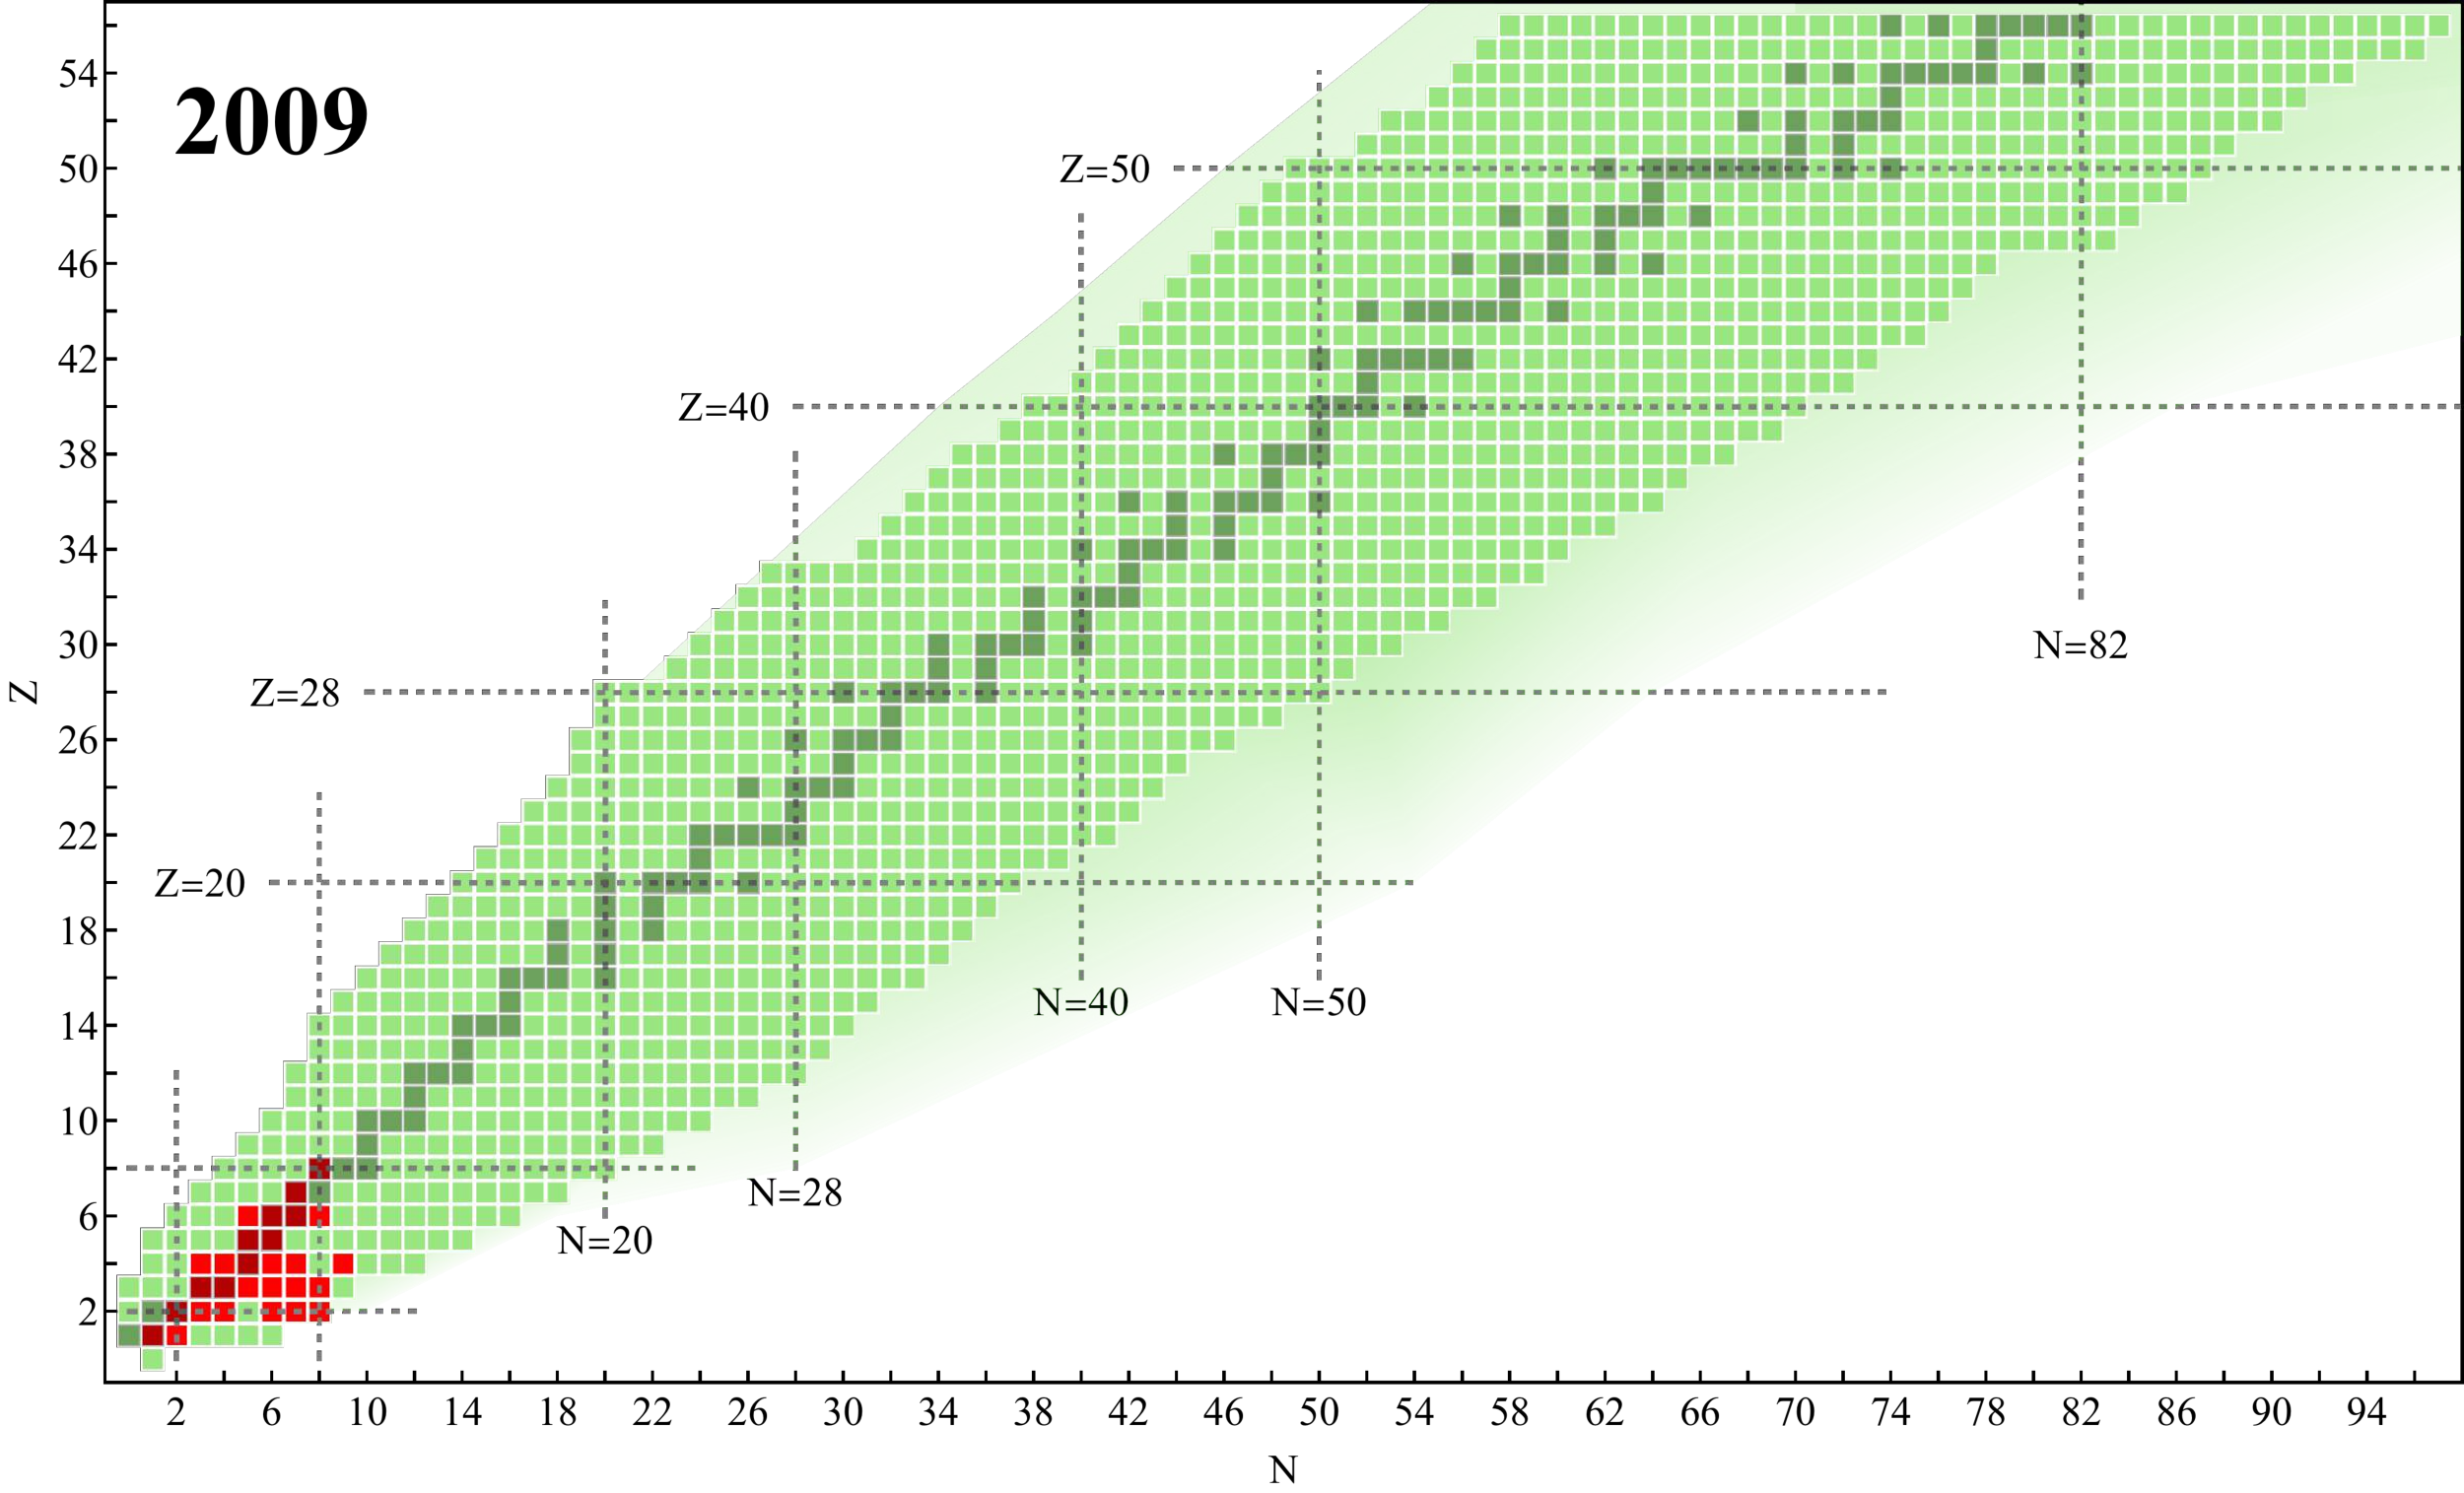
\includegraphics[width=0.45\textwidth]{proposal/doc/images/external/nuclear_chart_2009.pdf}
  \hspace{0cm}
  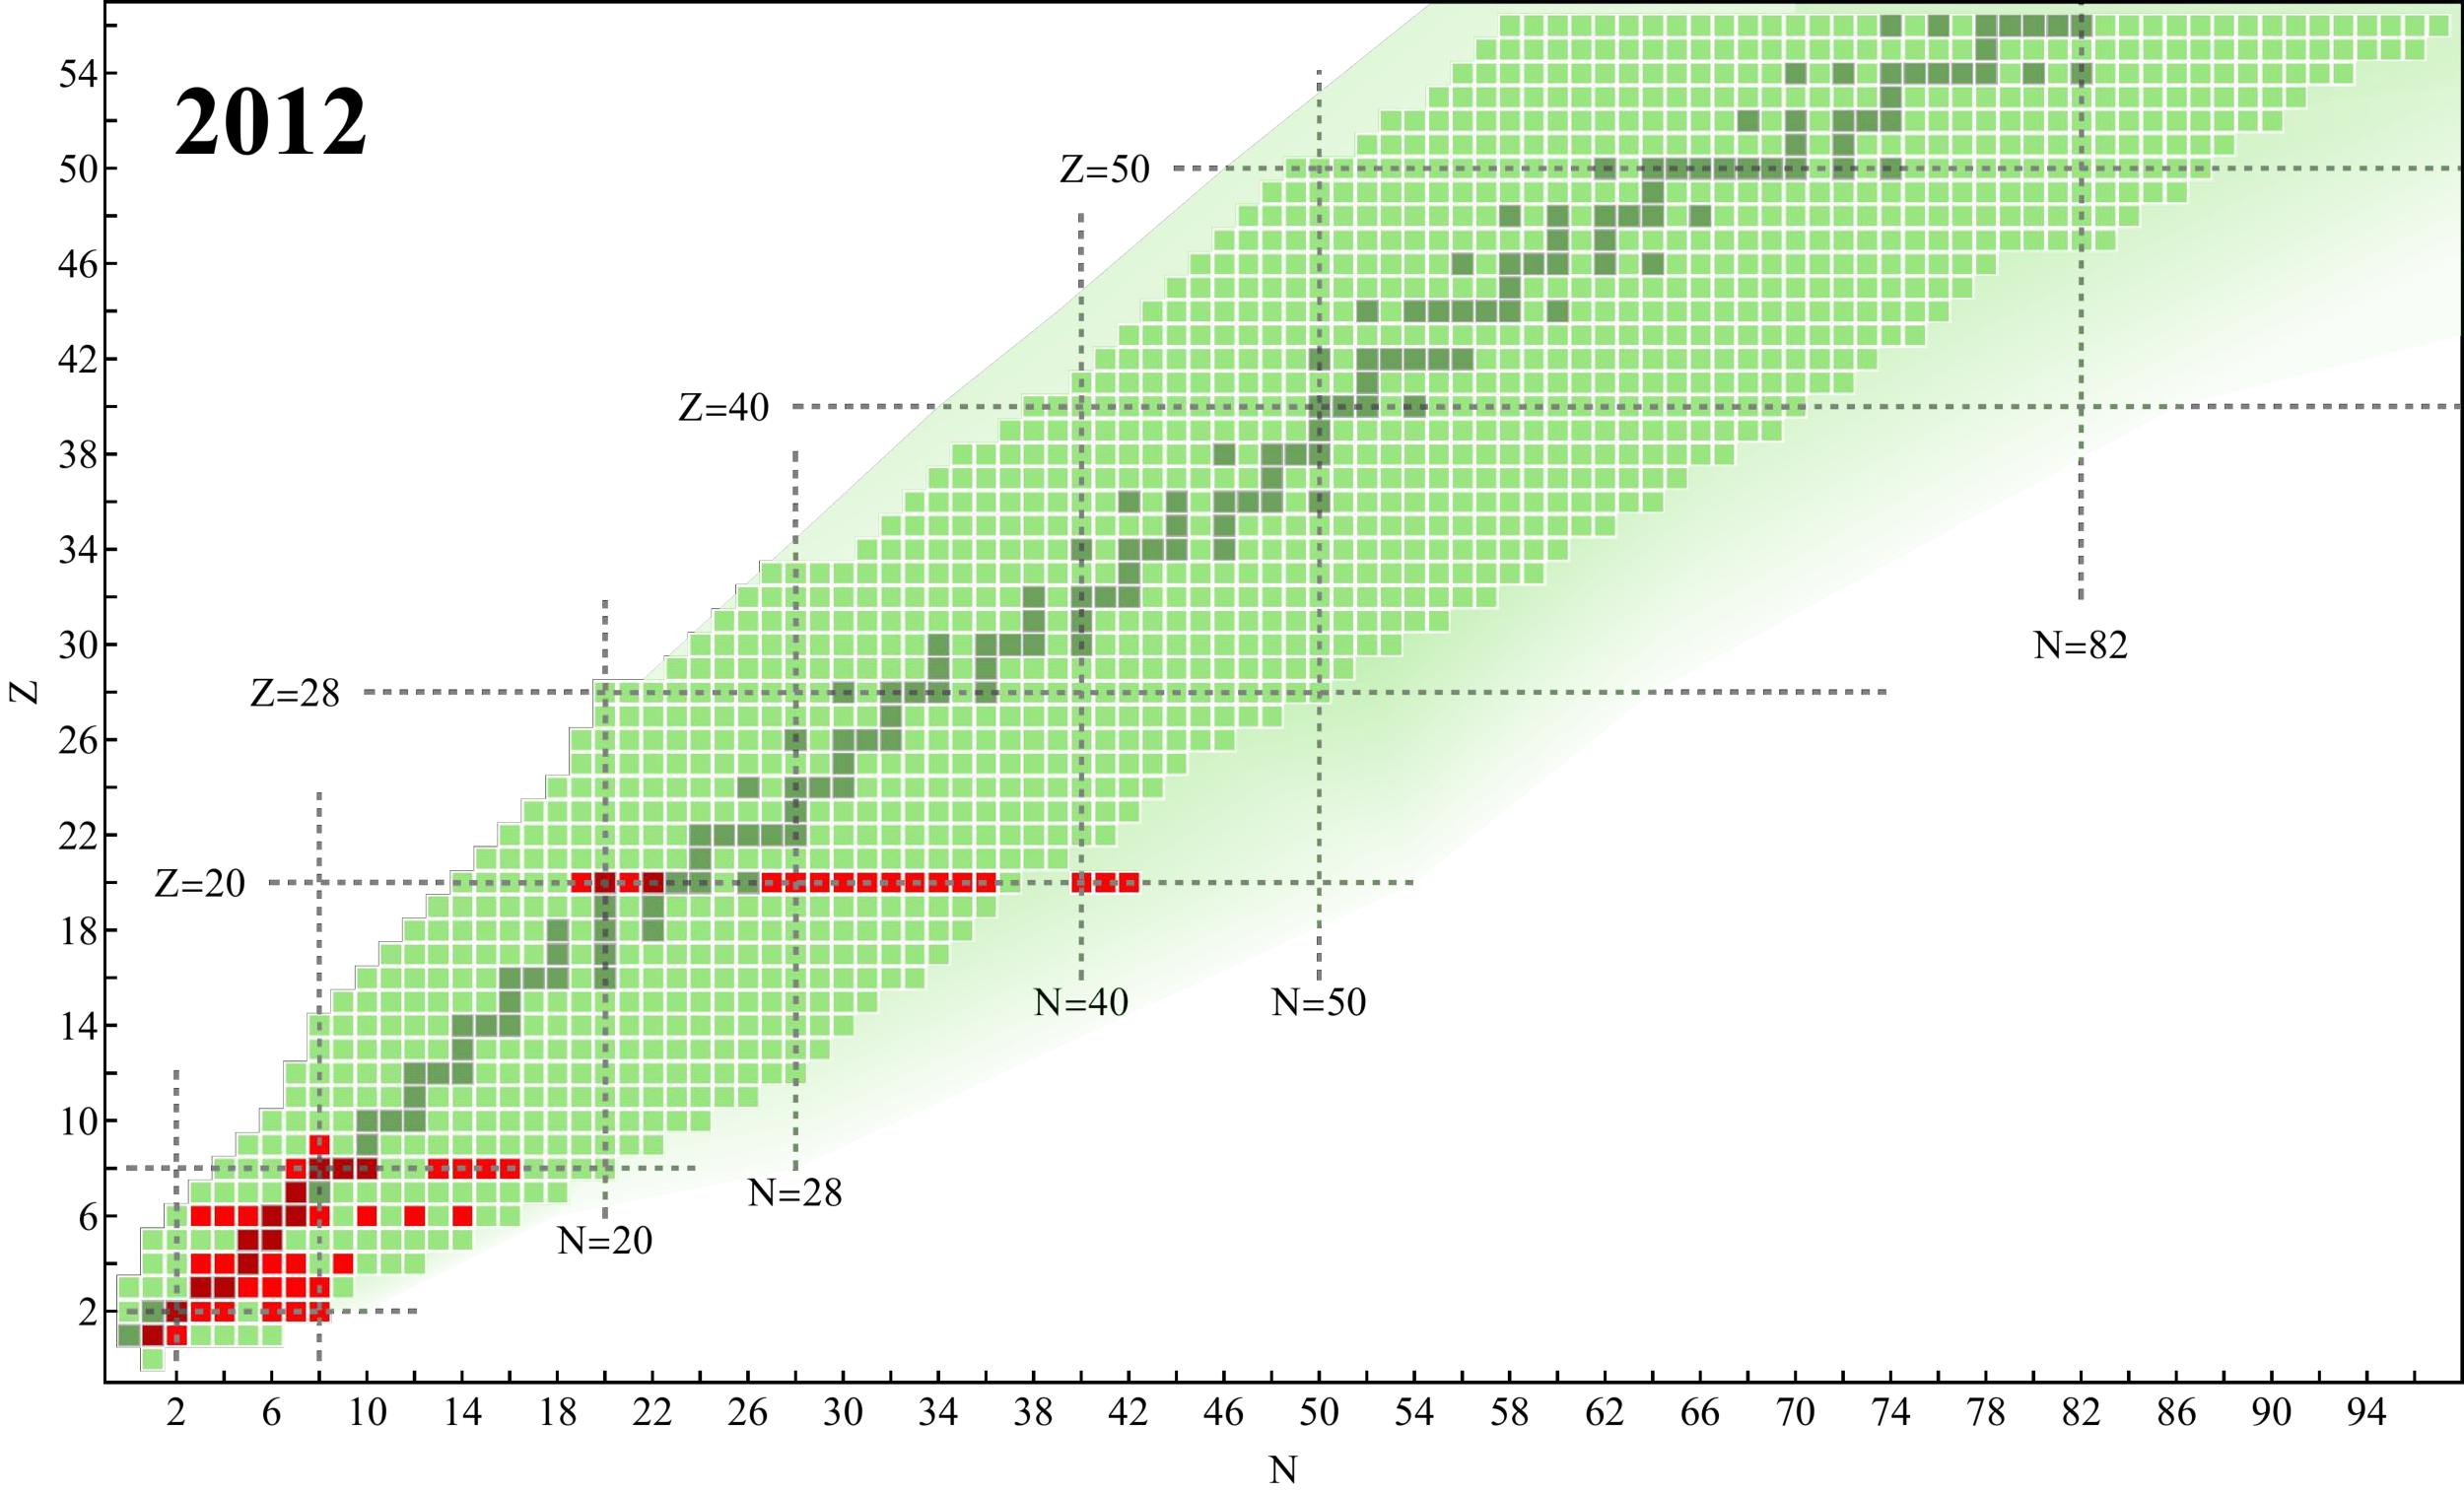
\includegraphics[width=0.45\textwidth]{proposal/doc/images/external/nuclear_chart_2012.pdf}\\
  \vspace{0.05cm}
  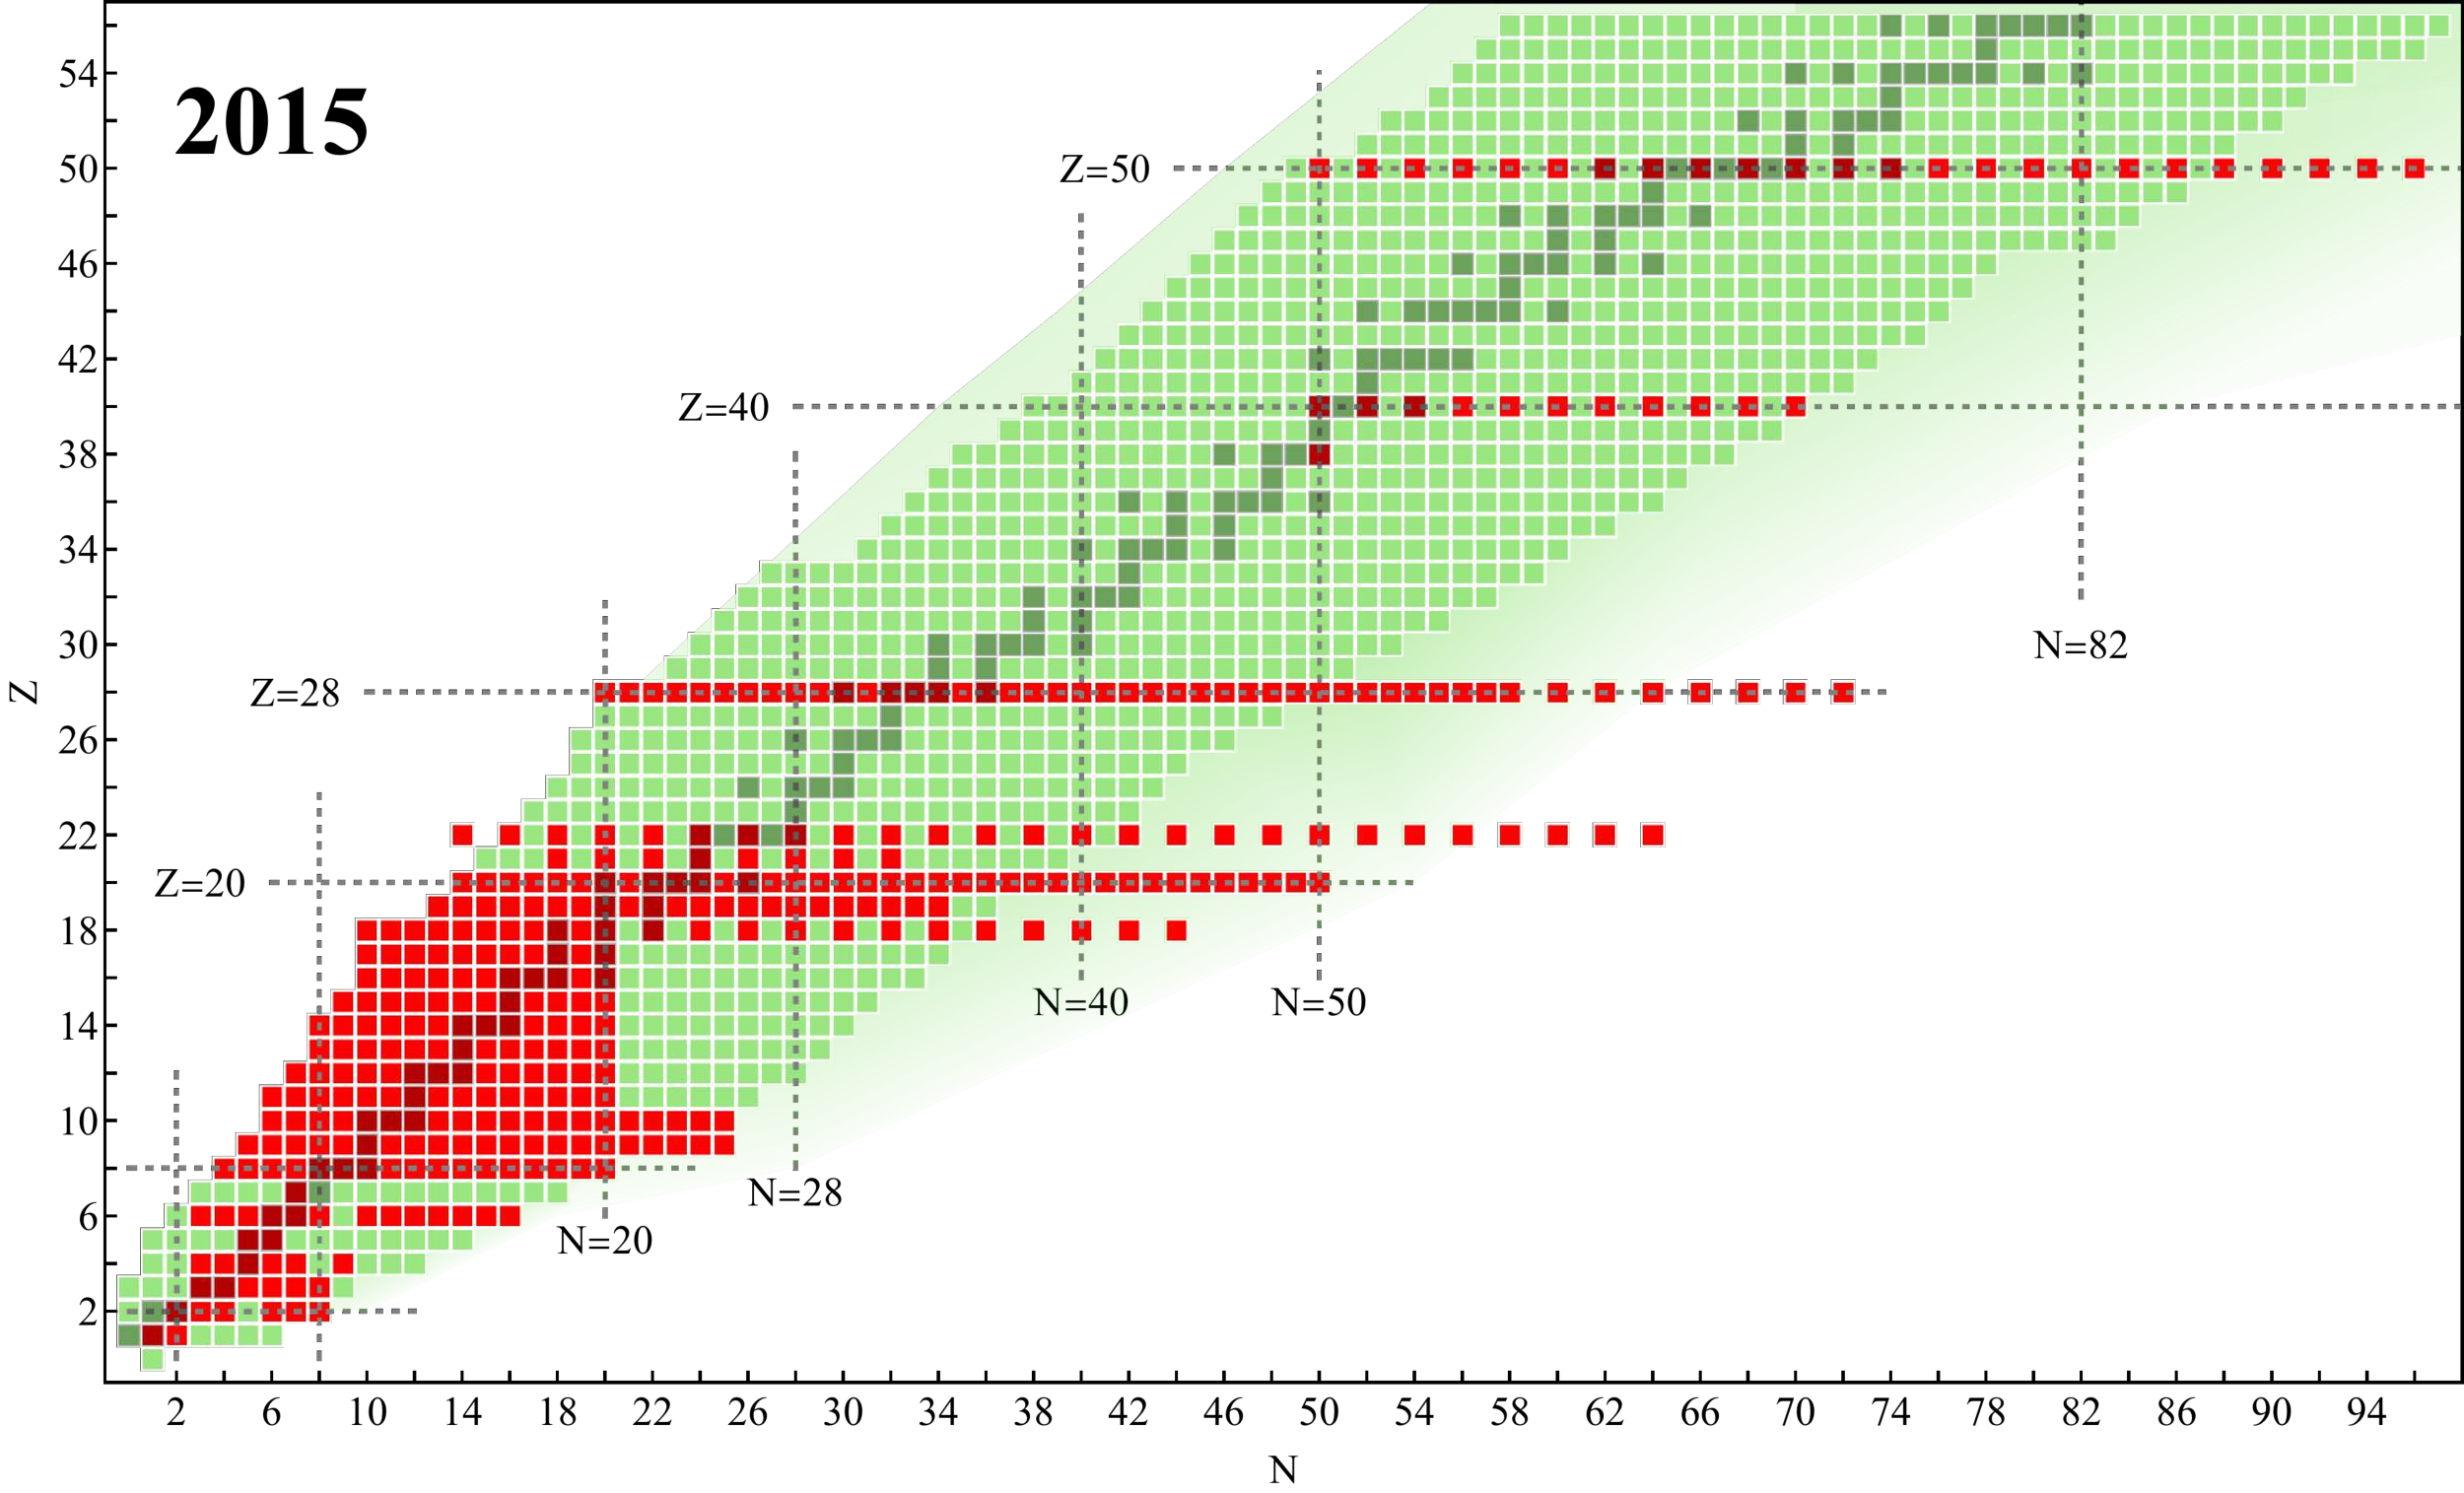
\includegraphics[width=0.45\textwidth]{proposal/doc/images/external/nuclear_chart_2015.pdf}
  \hspace{0cm}
  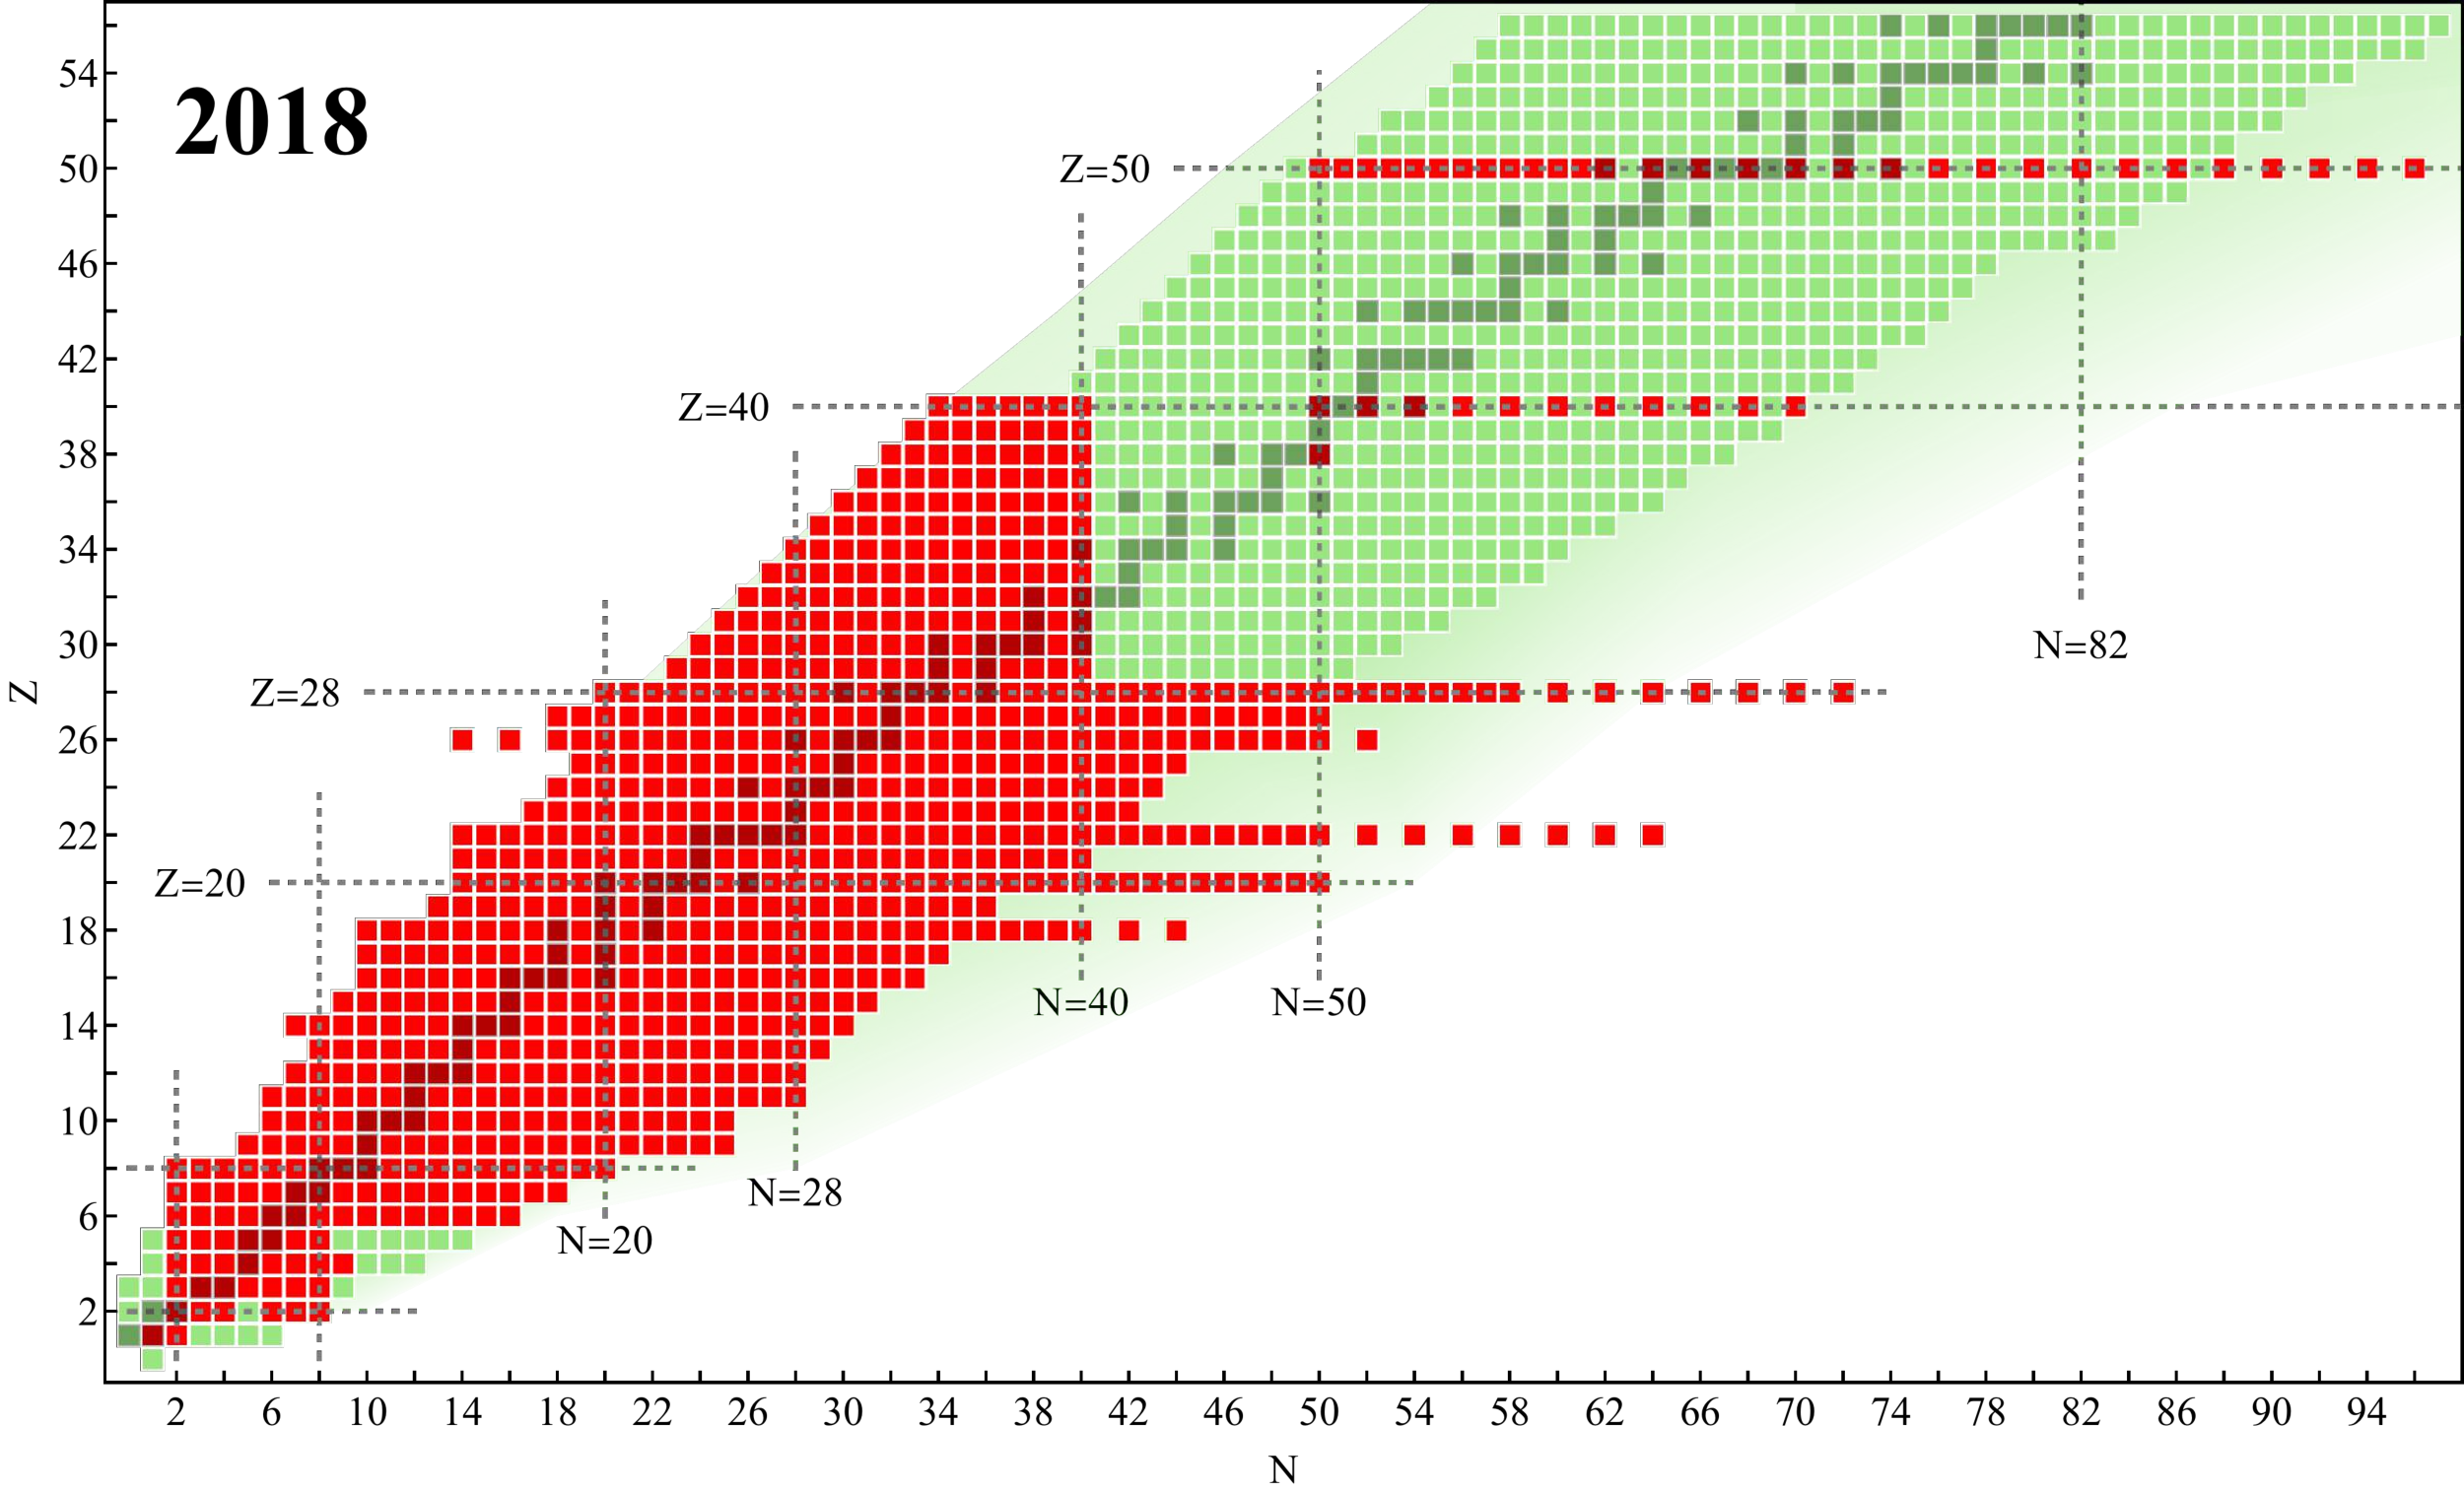
\includegraphics[width=0.45\textwidth]{proposal/doc/images/external/nuclear_chart_2018.pdf}
  \caption[
    Chart of nuclides showing in red nuclei for which \abinitio{} calculations
    involving two- and three-body interactions had been done in 2009 (top left)
    to 2018 (bottom right).
    Only calculations for which covergence with respect to basis size was achieved
    are included in the charts.
  ]{
    Chart of nuclides showing in red nuclei for which \abinitio{} calculations
    involving two- and three-body interactions had been done in 2009 (top left)
    to 2018 (bottom right).
    Only calculations for which covergence with respect to basis size was achieved
    are included in the charts.
    Figure courtesy of Heiko Hergert~\cite{Herg15imsrgphysrep}.
  }\label{fig:ab_initio_conquest}
\end{figure}

Over the past two decades,
the range of \abinitio{} results has expanded rapidly,
as is shown in Fig.~\ref{fig:ab_initio_conquest}.
This change was driven by shift in our understanding of \textit{low-energy}
nuclear physics,
encapsulated in the effective field theory (EFT) and renormalization group (RG) methods.
Underlying both of these ideas is the concept of limited resolution in low-energy physics
and the realization that behavior at short distances (small wavelengths or high energies)
does not affect the big picture at long distances.
Effective field theory methods connect to underlying fundamental theories
explicitly setting the scale to include essential long-distance physics
and generating the most general expansion for the short-distance physics
in terms of contact interactions~\cite{Wein78eft,Hamm19nuceftreview}.
Renormalization group methods allow for varying of the resolution scale,
decoupling or integrating out high-energy details to produce an efficient low-resolution
description of the system at hand~\cite{Wils71rg,Bogn06srg,Bogn09vlowk}.
These two obviously synergistic methods have worked together to produce
low-resolution nuclear forces rooted in the fundamental theory of quantum chromodynamics.

With these new, more efficient low-energy nuclear forces
and the ever increasing available computational resources,
the parallel development of nuclear many-body methods was uncapped.
New developments on old methods, such as coupled cluster,
and the introduction of new methods,
such as the in-medium similarity renormalization group,
have carried \abinitio{} nuclear theory to its present state.

\section{Goals}

The focus of this work will be the in-medium similarity renormalization group (IM-SRG)~\cite{Tsuk10imsrg}.
As indicated by its name,
it brings the RG approach of decoupling low- and high-energy states to the many-body problem,
seeking to decouple the state of a system from its excitations.
It is flexible in that it can target both ground states and low-lying excited states
and calculate energies as well as expectation values for other operators,
and while its original formulation centers on describing closed-shell nuclei,
multiple variants are able to model open-shell nuclei as well.

The current state-of-the-art IM-SRG approaches truncate the formalism at the IM-SRG(2) level,
the first non-trivial truncation where up to normal-ordered two-body operators are kept in the equations.
This truncation has been quite successful,
but for the purposes of reaching higher precision and allowing for quantification
of many-body uncertainties,
extending the truncation to the IM-SRG(3) level is of great interest.
In this work, we aim to systematically study the improvements offered by the IM-SRG(3)
for the ground-state properties of light and medium-mass nuclei.
As a step towards this goal,
we also consider the simpler pairing Hamiltonian system in the IM-SRG.\@

\section{Outline}

The remainder of this thesis is structured as follows:
\begin{itemize}
  \item{In Chapter~\ref{ch:nuclear_forces},
    we introduce some aspects of the theory of nuclear forces.
    We focus on the modern approaches to deriving nuclear forces
    and using choices to improve the convergence of many-body calculations.}
  \item{In Chapter~\ref{ch:many_body},
    we introduce the many-body formalism that underlies the IM-SRG.\@
    We introduce some other many-body methods that also build on this formalism
    to help position the IM-SRG in the greater space of available many-body methods.}
  \item{In Chapter~\ref{ch:imsrg},
    we discuss the IM-SRG in detail.
    We discuss the general formalism and the IM-SRG(2) and IM-SRG(3) truncations.
    We also discuss generator choice,
    which sets how the IM-SRG decouples low and high energies,
    and the Magnus expansion,
    an extension that makes it easier to solve and easier to apply to other observables.}
  \item{In Chapter~\ref{ch:results},
    we discuss the results of our application of our IM-SRG implementation.
    These results are primarily benchmarks to validate the correctness of our implementation.}
  \item{In Chapter~\ref{ch:summary},
    we summarize our results
    and offer an outlook for the next steps towards the goals of this thesis.}
\end{itemize}

